\documentclass[10pt, a5paper]{article}
\usepackage{pdfpages}
\usepackage{parallel}
\usepackage[T2A]{fontenc}
\usepackage{ucs}
\usepackage[utf8x]{inputenc}
\usepackage[polish,english,russian]{babel}
\usepackage{hyperref}
\usepackage{rotating}
\usepackage[inner=2cm,top=1.8cm,outer=2cm,bottom=2.3cm,nohead]{geometry}
\usepackage{listings}
\usepackage{graphicx}
\usepackage{wrapfig}
\usepackage{longtable}
\usepackage{indentfirst}
\usepackage{array}
\newcolumntype{P}[1]{>{\raggedright\arraybackslash}p{#1}}
\frenchspacing
\usepackage{fixltx2e} %text sub- and superscripts
\usepackage{icomma} % коскі ў матэматычным рэжыме
\PreloadUnicodePage{4}

\newcommand{\longpage}{\enlargethispage{\baselineskip}}
\newcommand{\shortpage}{\enlargethispage{-\baselineskip}}

\def\switchlang#1{\expandafter\csname switchlang#1\endcsname}
\def\switchlangbe{
\let\saverefname=\refname%
\def\refname{Літаратура}%
\def\figurename{Іл.}%
}
\def\switchlangen{
\let\saverefname=\refname%
\def\refname{References}%
\def\figurename{Fig.}%
}
\def\switchlangru{
\let\saverefname=\refname%
\let\savefigurename=\figurename%
\def\refname{Литература}%
\def\figurename{Рис.}%
}

\hyphenation{admi-ni-stra-tive}
\hyphenation{ex-pe-ri-ence}
\hyphenation{fle-xi-bi-li-ty}
\hyphenation{Py-thon}
\hyphenation{ma-the-ma-ti-cal}
\hyphenation{re-ported}
\hyphenation{imp-le-menta-tions}
\hyphenation{pro-vides}
\hyphenation{en-gi-neering}
\hyphenation{com-pa-ti-bi-li-ty}
\hyphenation{im-pos-sible}
\hyphenation{desk-top}
\hyphenation{elec-tro-nic}
\hyphenation{com-pa-ny}
\hyphenation{de-ve-lop-ment}
\hyphenation{de-ve-loping}
\hyphenation{de-ve-lop}
\hyphenation{da-ta-ba-se}
\hyphenation{plat-forms}
\hyphenation{or-ga-ni-za-tion}
\hyphenation{pro-gramming}
\hyphenation{in-stru-ments}
\hyphenation{Li-nux}
\hyphenation{sour-ce}
\hyphenation{en-vi-ron-ment}
\hyphenation{Te-le-pathy}
\hyphenation{Li-nux-ov-ka}
\hyphenation{Open-BSD}
\hyphenation{Free-BSD}
\hyphenation{men-ti-on-ed}
\hyphenation{app-li-ca-tion}

\def\progref!#1!{\texttt{#1}}
\renewcommand{\arraystretch}{2} %Іначай формулы ў матрыцы зліпаюцца з лініямі
\usepackage{array}

\def\interview #1 (#2), #3, #4, #5\par{

\section[#1, #3, #4]{#1 -- #3, #4}
\def\qname{LVEE}
\def\aname{#1}
\def\q ##1\par{{\noindent \bf \qname: ##1 }\par}
\def\a{{\noindent \bf \aname: } \def\qname{L}\def\aname{#2}}
}

\def\interview* #1 (#2), #3, #4, #5\par{

\section*{#1\\{\small\rm #3, #4. #5}}

\def\qname{LVEE}
\def\aname{#1}
\def\q ##1\par{{\noindent \bf \qname: ##1 }\par}
\def\a{{\noindent \bf \aname: } \def\qname{L}\def\aname{#2}}
}

\begin{document}
\title{Многослойные и многоуровневые системы хранения данных.\footnote{\url{alex_kls@mail.ru} \url{http://lvee.org/ru/abstracts/238}}}
\author{Александр Клыга, Minsk, Belarus}
\maketitle
\begin{abstract}
In multilayers data storages the storage drivers are grouped into
separate layers according to their technical characteristics. The first layer contains high-speed solid-state drivers (SSDs), whereas the other layers can have HDDs or others storage devices (tape, optical devices). The multilayer data storage provides high speed data access and can be formed by using hardware or software solutions. In multilevel software-define storages (SDS), the separate data storage are grouped with respect to levels of their technical characteristics, the type of stored data, and availability requirements for the end user. Multilevels SDS allows for optimization of the data placement in the storage. The main node of SDS is represented by a controller. The SDS controller is a software platform (open source and other) which includes solution tools for management, monitoring and migration of data between layers.
\end{abstract}
\subsection*{Многослойные и многоуровневые системы хранения данных. Обзор архитектуры и решений на базе open source.}

В настоящее время развитие систем хранения данных (СХД) обусловлено следующими тенденциями (по материалам конференции ~\cite{kliga-1}):

\begin{itemize}
  \item постепенно разработка новых накопителей для хранения данных на базе магнитных дисков замедляется, при этом отмечаются технологические проблемы с производством дисков большой емкости;
  \item стремительное развитие технологий производства устройств хранения данных на базе flash памяти. При этом их емкость  постоянно увеличиваются, а надежность хранения данных гарантируется на высоком уровне;
  \item цена устройств на базе flash памяти больше не является сдерживающим фактором их применения в системах хранения данных;
  \item использованием нового интерфейса NVM Express (NVMe, \linebreak NVMHCI -- Non-Volatile Memory Host Controller Interface \linebreak Specification ~\cite{kliga-2}) для твердотельных устройств хранения данных (SSD);
  \item использование решений с открытым кодом для  построения программно-определяемых систем хранения данных.
\end{itemize}

Популярным архитектурным решением СХД являются многослойные хранилища данных разработанные на базе технологии  тиринга (от анг. tiering) и использующие интеллектуальные алгоритмы распределения данных между слоями. В основе технологии тиринга лежит принцип разделения хранилища данных на слои, отличающихся производительностью в зависимости от используемых типов запоминающих устройств, из которых оно состоит (например, твердотельные диски SSD или разноскоростные шпиндельных HDD). Для управления размещением данных по слоям СХД могут использоваться как аппаратные решения, например, RAID контроллеры с поддержкой технологии тиринга, так и различные  программные решения (в том числе на базе open source). Одним из преимуществ использования программных решений является, то что в качестве слоев могут быть использованы дополнительные хранилища данных подключенные к контроллеру СХД.

При многоуровневом построении СХД отдельные хранилища данных группируются по уровням на основании их технических характеристик, типа хранимых данных, и требований доступности для конечного потребителя. Многоуровневые СХД, как правило, реализуются виде программно-определяемых систем хранения данных или software-define storages (SDS).

\subsection*{Многослойные  системы хранения данных.}

Технология тиринга применяемая при создании многослойных СХД позволяет группировать устройства хранения данных в отдельные слои в зависимости от их типа и характеристик. Для улучшения производительности хранилища данных между сломи могут располагаться дополнительные cache-layer, основное назначение которых повышение производительности при миграции данных между слоями, или уменьшение латентности отклика данных между  пространством пользователя и СХД. Общая структура СХД  с многослойной структурой приведена на рисунке ниже.

\begin{center}

\begin{figure}[h!]
  \centering
  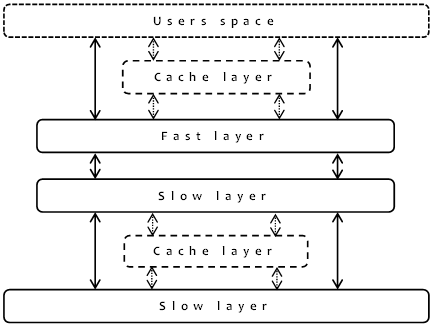
\includegraphics[width=4cm]{kliga1.jpg}
  
  \label{Kliga1}
\end{figure}

\end{center}

Обычно в качестве cache-layer используют RAM-диски созданные в ОЗУ или SSD диски, если необходимо кэширование между  слоями с медленными накопителями. В слой fast-layer, как правило, объединяют быстрые диски, типа SSD, но при этом важно учитывать их технические характеристики. Так, например, при использовании SSD с интерфейсом  NVMe, рекомендуется делать несколько слоев  fast-layer, объединяя в каждый слой SSD накопители одного типа.  В слои slow-layer как правило, объединяют шпиндельные накопители на магнитных дисках (HDD), группируя исходя из их технических характеристик, либо иные типы накопителей, например, ленточные.

Суммарный объем многослойного СХД равен сумме объемов каждого слоя, при этом необходимо учитывать, что по мере заполнения слоя данными, часть его объема может быть зарезервировано для операций миграции данных (до 5\% или более от общей емкости слоя).

Существуют две основные концепции создания многослойных СХД с использованием программных решений.  В рамках первой концепции с помощью программных средств установленных на контроллере СХД для пространства пользователя создается интерфейс доступа к хранилищу данных как устройства блочного типа, таким образом пользователь оперирует с ним как с обычным накопителем. Управление контроллером СХД осуществляется через программный интерфейс, а структура слоев скрыта от пользователя.

В рамках второй концепции возможности создания многослойных СХД реализуется с помощью программного менеджера накопителей в файловой системе (наиболее популярное решения для  хранилища данных модели DAS). Такой подход реализованы, например, в файловых системах как Bcachefs ~\cite{kliga-3}, ZFS ~\cite{kliga-4} и Btrfs ~\cite{kliga-5}. Основным преимуществом этой концепции является то, что пользователь может полностью управлять как слоями так и накопителями в СХД.

Так же важно отметить, что технологии тиринга и кэширования широко  используются в решениях программных систем хранения данных, например, в распределенной файловой системе GlusterFS ~\cite{kliga-7}, или объектном хранилище данных Ceph ~\cite{kliga-6}.

\subsection*{Многоуровневые  системы хранения данных.}

В основу концепции многоуровневых систем хранения данных положен принцип объединения отдельных хранилищ данных в единую СХД с общим центром управления и мониторинга, основанную на модели программно-определяемых  систем хранения данных (software-define storage или SDS). Основным компонентом многоуровневого СХД является контроллер, который осуществляет мониторинг и анализ статистики работы отдельных хранилищ данных, управляем миграцией между уровнями, и обеспечивает подключение новых хранилищ к СХД.  Общая структурная схема многоуровневого СХД приведена ниже.

\begin{center}

\begin{figure}[h!]
  \centering
  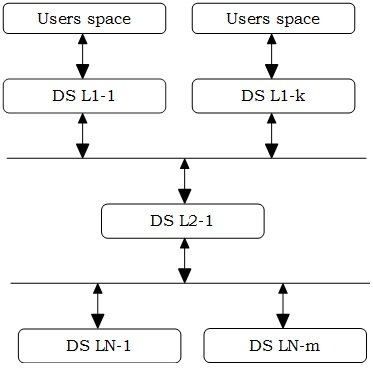
\includegraphics[width=4cm]{kliga2.jpg}
  
  \label{Kliga2}
\end{figure}

\end{center}


\begin{center}\end{center}

На верхнем уровне, как правило, располагают хранилища данных взаимодействующим с пространством пользователя. На втором уровне, как правило, располагают хранилища данных основное назначение которых хранить «холодные данные» с хранилищ первого уровня, и поддерживать миграцию данных между ними. На третьем и ниже уровне могут находится хранилища архивных данных. Основным преимуществом такой модели СХД является оптимизация хранения данных на первом уровне и распределение нагрузки между хранилищами.

Для реализации многоуровневых СХД могут быть использованы различные программные решения, например, в качестве контроллера может быть использован open source проект CorpHD ~\cite{kliga-8}. Одним из его преимуществ является интеграция с объектным хранилищем данных Ceph, и гибкая настройка архитектуры.

Программно-определяемые хранилища данных являются перспективным направлением развития систем хранения данных и поэтому  Linux Foundation в октябре прошлого года объявил о старте нового проекта по созданию Open Controller for Software-Defined Storage ~\cite{kliga-9}, который станет основой для построения открытых решений SDS. Ознакомится с этим новым проектом можно на его официальном ресурсе ~\cite{kliga-10}.

%\subsection*{Ссылки}
\begin{thebibliography}{20}
\bibitem{kliga-1}Flash memory summit \url{https://www.flashmemorysummit.com/}
\bibitem{kliga-2}The official site NVM Express: // \url{http://www.nvmexpress.org/}
\bibitem{kliga-3}Bcachefs: An advanced new filesystem for Linux // \url{http://bcachefs.org/}
\bibitem{kliga-4}ZFS: Zettabyte File System (OpenZFS project) //  \url{http://open-zfs.org/}
\bibitem{kliga-5}Btrfs: Btrfs is a modern CoW filesystem for Linux // \url{https://btrfs.wiki.kernel.org/index.php/Main_Page}
\bibitem{kliga-6}Ceph: The future of storage // \url{https://ceph.com/}
\bibitem{kliga-7}Gluster: Storage for your Cloud // \url{https://www.gluster.org/}
\bibitem{kliga-8}CorpHD: An open source software defined storage controller // \url{https://coprhd.github.io/}
\bibitem{kliga-9}The Linux Foundation creates Open Controller for Software-Defined Storage // \url{https://www.linuxfoundation.org/announcements/linux-foundation-creates-open-controller-for-_software-defined-storage}
\bibitem{kliga-10}OpenSDS Project // \url{https://www.opensds.io/}
\end{thebibliography}

\end{document}
